\chapter{Конструкторская часть}

\section{Разработка алгоритмов}

На рисунках~\ref{fig:levRec},~\ref{fig:levMem},~\ref{fig:levItr}~и~\ref{fig:damItr} представлены схемы алгоритмов. На вход каждому из алгоритмов подаются строки first и second длиной n и m соответственно. Алгоритм с мемоизацией также получает матрицу cache размером n+1 на m+1.

\begin{figure}[h!]
	\centering
	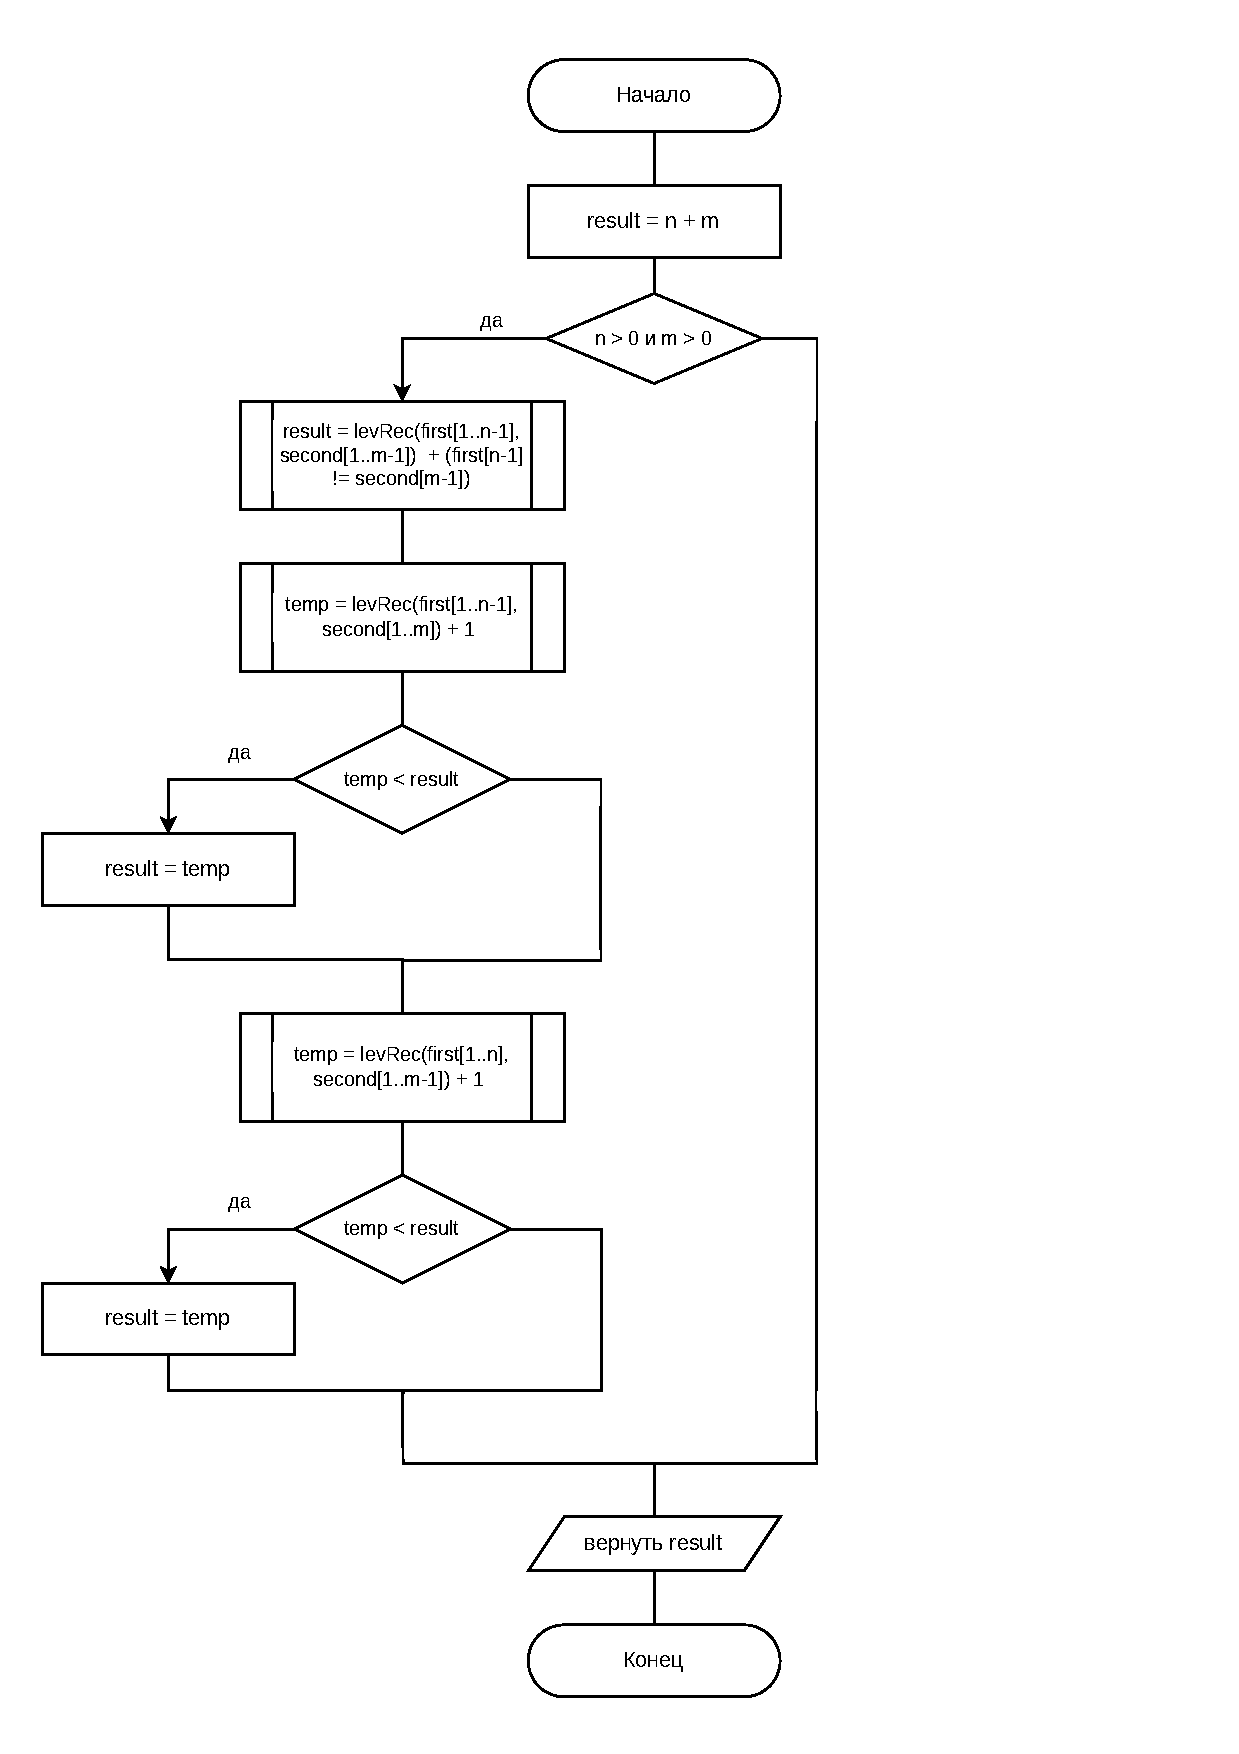
\includegraphics[height=0.6\textheight]{tex_parts/scheme1.pdf}
	\caption{\label{fig:levRec}Схема рекурсивного алгоритма нахождения расстояния Левенштейна}
\end{figure}

\clearpage

\begin{figure}[h!]
	\centering
	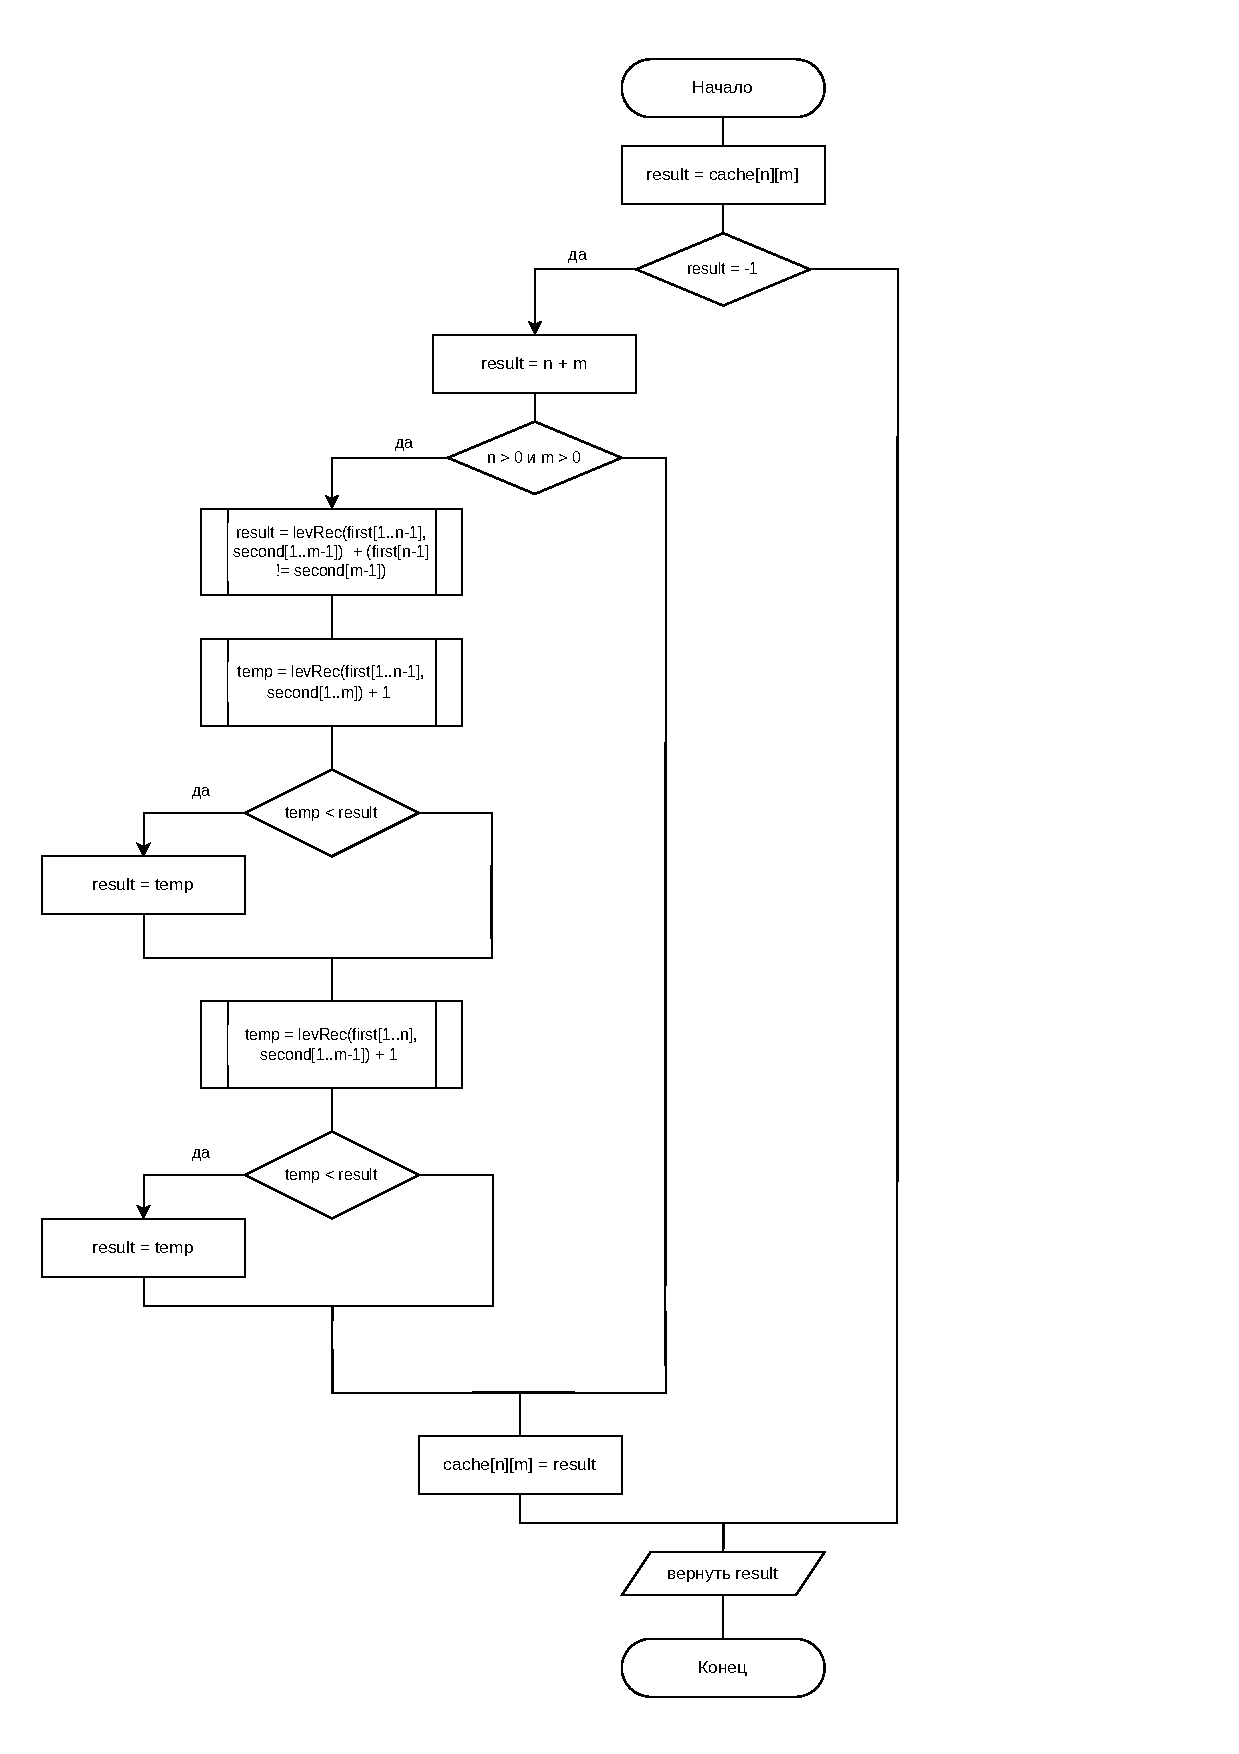
\includegraphics[height=0.8\textheight]{tex_parts/scheme2.pdf}
	\caption{\label{fig:levMem}Схема рекурсивного алгоритма нахождения расстояния Левенштейна с мемоизацией}
\end{figure}

\clearpage

\begin{figure}[h!]
	\centering
	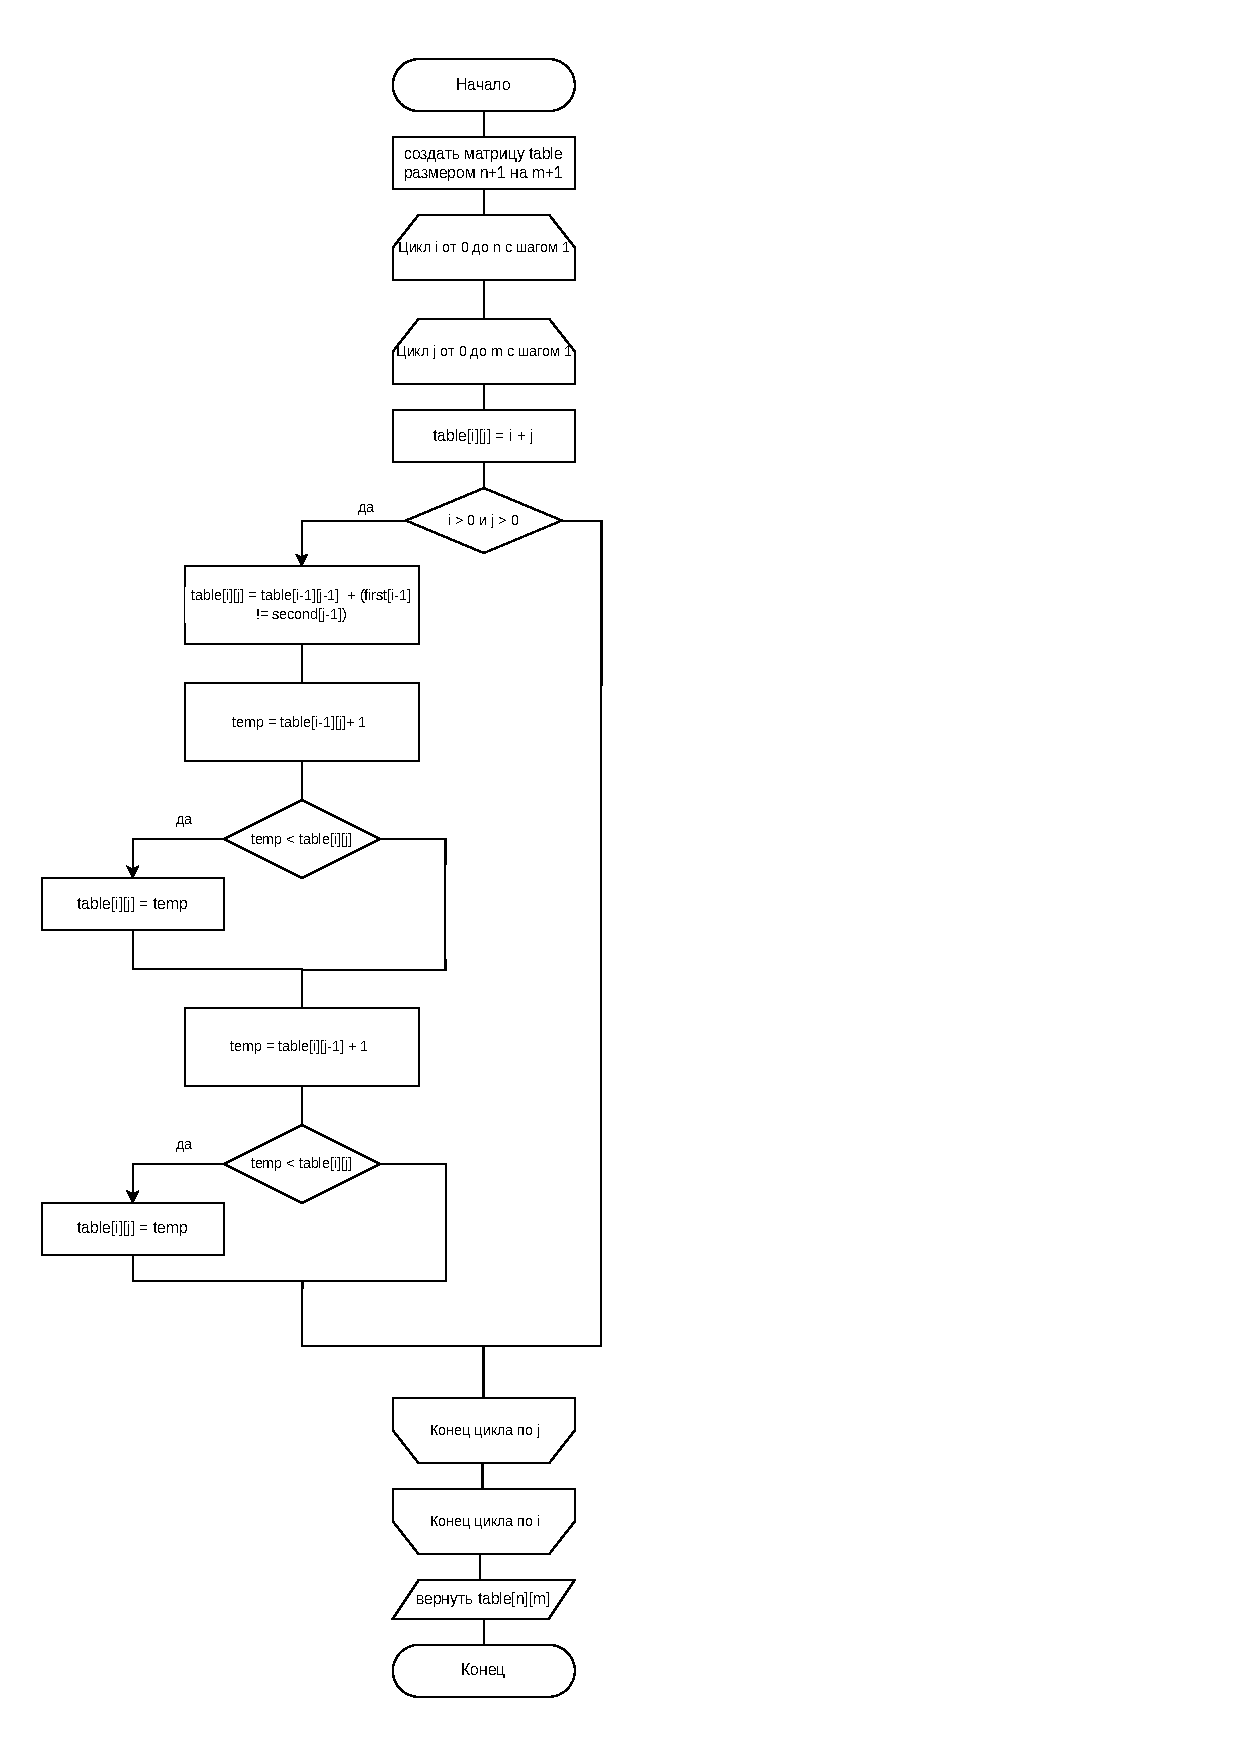
\includegraphics[height=0.8\textheight]{tex_parts/scheme3.pdf}
	\caption{\label{fig:levItr}Схема матричного алгоритма нахождения расстояния Левенштейна}
\end{figure}

\clearpage

\begin{figure}[h!]
	\centering
	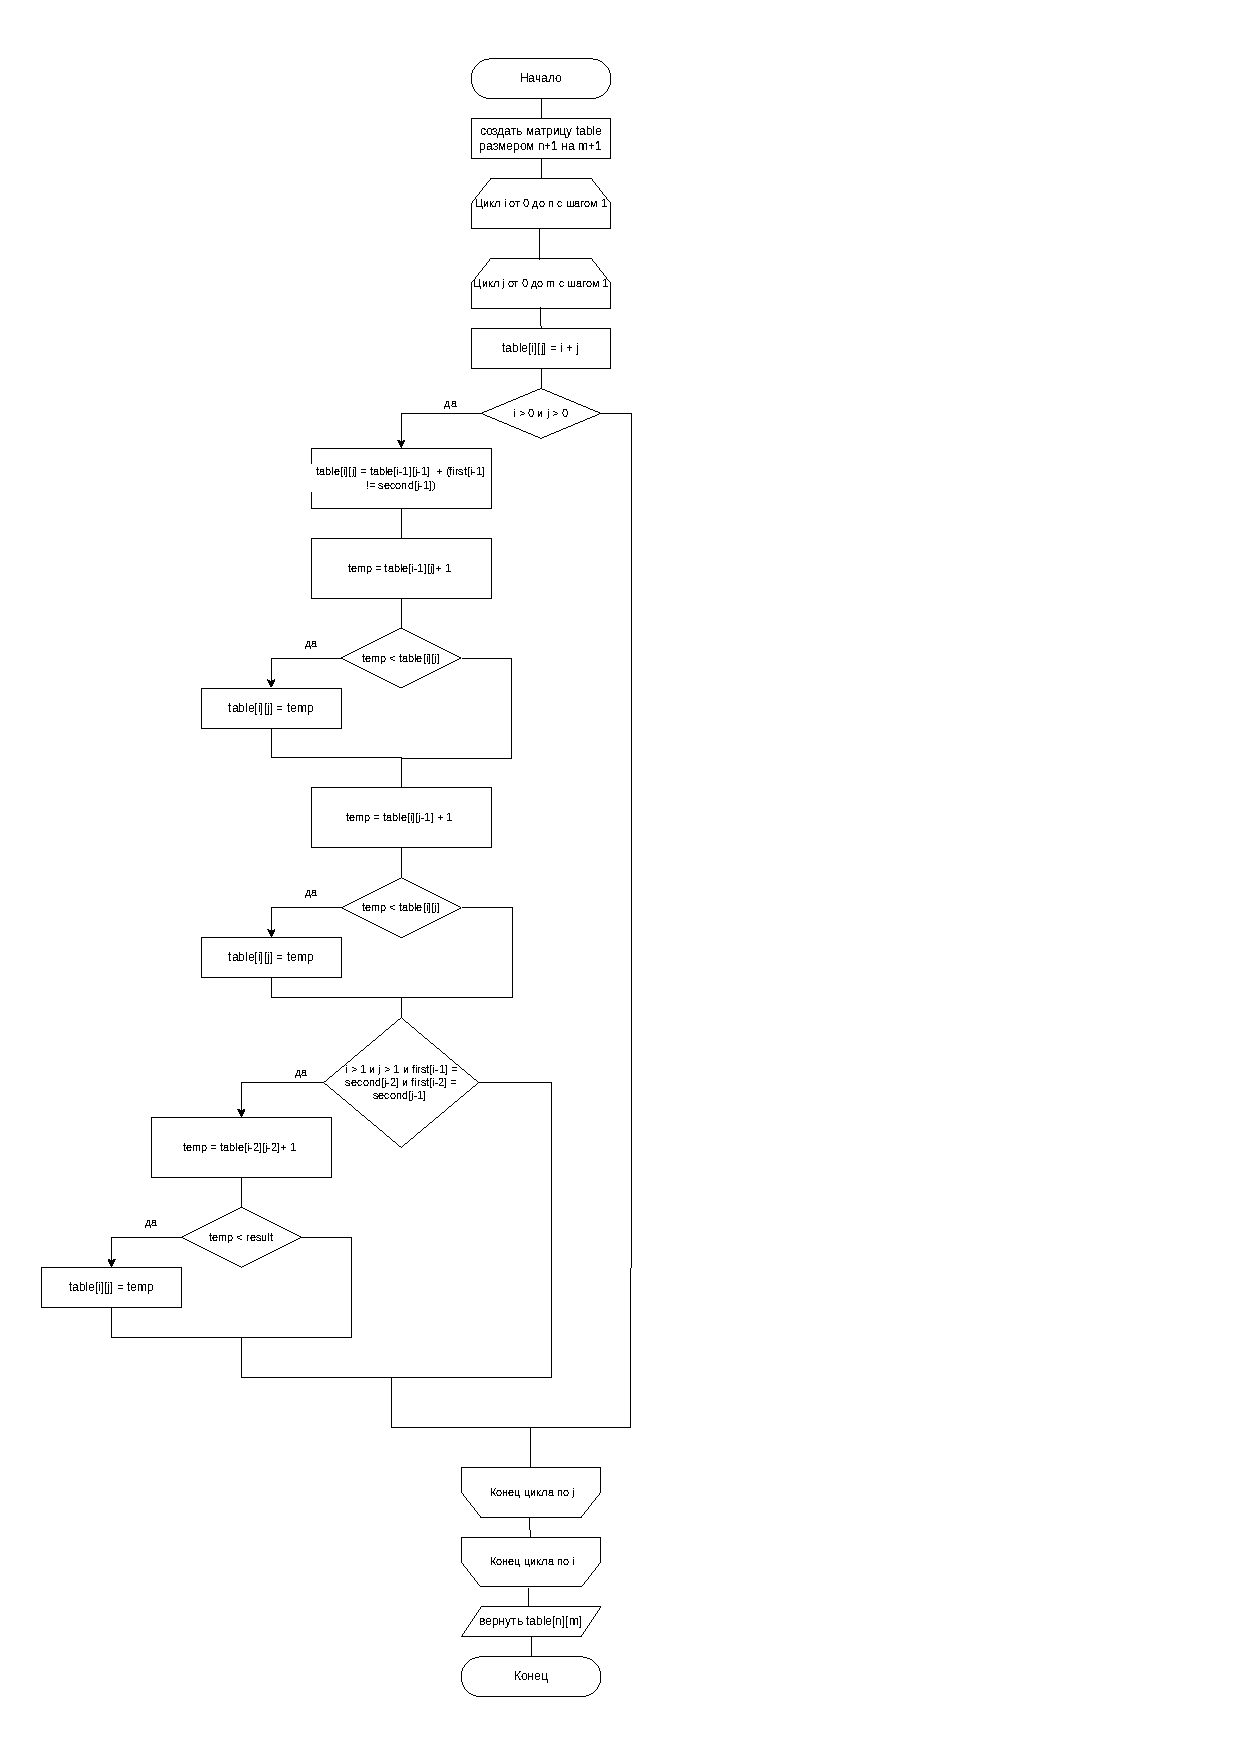
\includegraphics[height=0.8\textheight]{tex_parts/scheme4.pdf}
	\caption{\label{fig:damItr}Схема матричного алгоритма нахождения расстояния Дамерау-Левенштейна}
\end{figure}

\clearpage

\section{Используемые типы и структуры данных}

При реализации алгоритмов использованы следующие структуры данных:

\begin{itemize}
	\item строка -- массив символов;
	\item длина строки -- целое беззнаковое число;
	\item матрица -- двумерный массив целых чисел.
\end{itemize}

\section{Выводы}

В данном разделе были построены схемы алгоритмов и выбраны структуры данных.

